\documentclass{standalone}

\usepackage{standalone}
\usepackage{tikz}
\usetikzlibrary{er,positioning, calc}

\begin{document}

	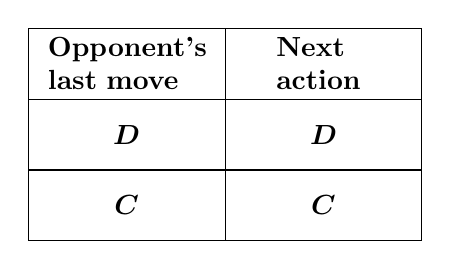
\begin{tikzpicture}
    	\tikzstyle{state}=[minimum width=2.5cm, minimum height=0.9cm, font=\boldmath];

       \node[rectangle, draw=black, text width=2cm] (0) at (0, 0) [state] 
       {\textbf{Opponent's last move}};

    \node[rectangle, draw=black] (3) at (0, -0.9) [state] {$D$};
    \node[rectangle, draw=black] (3) at (0, -1.8) [state] {$C$};
    \node[rectangle, draw=black, text width=1.2cm] (0) at (2.5, 0) [state] 
    {\textbf{Next action}};
    \node[rectangle, draw=black] (3) at (2.5, -0.9) [state] {$D$};
    \node[rectangle, draw=black] (3) at (2.5, -1.8) [state] {$C$};
 
	\end{tikzpicture}
\end{document}